\documentclass[sigconf, numbers]{acmart}
\usepackage{booktabs}


%% \BibTeX command to typeset BibTeX logo in the docs
\AtBeginDocument{%
  \providecommand\BibTeX{{%
    \normalfont B\kern-0.5em{\scshape i\kern-0.25em b}\kern-0.8em\TeX}}}

%% These commands are for a PROCEEDINGS abstract or paper.
\settopmatter{printacmref=false} % Removes citation information below abstract
\renewcommand\footnotetextcopyrightpermission[1]{} % removes footnote with conference information in 

\acmConference[AEPRO 2026]{AEPRO 2026: Algorithm Engineering Projects}{March 1}{Jena, Germany}

% convert text to title case
% http://individed.com/code/to-title-case/

% that helps you to formulate your sentences
% https://www.deepl.com/translator

\begin{document}

%%
%% The "title" command has an optional parameter,
%% allowing the author to define a "short title" to be used in page headers.
\title[Enhancer for Scanned Images]{Enhancer for Scanned Images\\\large Algorithm Engineering 2026 Project Paper}

%%
%% The "author" command and its associated commands are used to define
%% the authors and their affiliations.

\author{Luca-Philipp Grumbach}
\affiliation{%
  \institution{Friedrich Schiller University Jena}
  \country{Germany}}
\email{max.mustermann@uni-jena.de}

\author{Lucas Obitz}
\affiliation{%
  \institution{Friedrich Schiller University Jena}
  \country{Germany}}
\email{lucas.obitz@uni-jena.de}

%% The abstract is a short summary of the work to be presented in the article.
\begin{abstract}

  Image denoising and binarization are fundamental preprocessing tasks in image processing. 
  This paper investigates adaptive thresholding techniques for producing clean black-and-white representations of noisy color images, with a focus on efficient processing of PPM image data.
  We implement and compare several classical local thresholding methods including Niblack, Sauvola, and Nick, as well as more modern adaptive approaches proposed by Bradley and Roth and by Bataineh et al.
  All methods are evaluated with respect to binarization quality, robustness to different window sizes, and computational performance.
  Our results show that modern integral image based approaches achieve superior foreground-background separation.
  In addition, profiling-guided optimizations demonstrate that integral images substantially reduce redundant sliding-window computations, leading to significant runtime improvements.
  These findings emphasize the importance of efficient local statistics computation for scalable adaptive thresholding.

\end{abstract}

%%
%% Keywords. The author(s) should pick words that accurately describe
%% the work being presented. Separate the keywords with commas.
\keywords{binarization, integral image processing, ppm, optimizations, parallelism}


%%
%% This command processes the author and affiliation and title
%% information and builds the first part of the formatted document.
\maketitle

\let\thefootnote\relax\footnotetext{AEPRO 2026, March 1, Jena, Germany. Copyright \copyright 2026 for this paper by its authors. Use permitted under Creative Commons License Attribution 4.0 International (CC BY 4.0).}

%--------------------------------------------%
% INTRODUCTION ------------------------------%
%--------------------------------------------%
\section{Introduction}\label{sec:introduction}

Reducing image noise is a fundamental problem in image processing, as noise can hide relevant structures and hinder subsequent analysis or interpretation. 
Images affected by sensor artifacts, compression errors, or non-uniform illumination often require preprocessing to enhance visual clarity and to improve the separability of foreground and background content.

In this work, we investigate the denoising and binarization of noisy color images, with the goal of producing clean black-and-white representations in the Portable Pixmap (PPM) image format and in JPEG.
We focus on adaptive and local thresholding techniques and examine how these methods can be efficiently applied to these color images.
To address the mentioned challenges, we employ established thresholding and denoising techniques and adapt them to operate efficiently on color image data. 

We approach this comparison by using the established mathematical formulations for local and adaptive thresholding. 
These methods are implemented and evaluated with respect to both denoising quality and computational efficiency.

\subsection{Background}\label{subsec:background}

The JPEG format is a widely used and well-understood standard for compressed image storage. 
In contrast, the PPM format is less commonly used in practice but is highly relevant in experimental contexts.
PPM images store uncompressed pixel data in a simple and explicit representation, allowing direct access to color values without the need for complex decoding.

These properties make PPM a suitable format for studying low-level image processing algorithms, as the distinct transformation of each pixel is possible.
Therefore, understanding the structure and limitations of the PPM format is essential for designing correct and efficient denoising and binarization algorithms.

\subsection{Related Work}\label{subsec:related}

Numerous approaches have been proposed for image denoising and binarization.
Classical methods include the local thresholding techniques introduced by Niblack~\cite{Niblack1985}, Sauvola et al.~\cite{Sauvola1997} and Khurshid et al.~\cite{Khurshid2009}.
These methods compute pixel-wise thresholds based on local image statistics such as the mean and standard deviation, with later approaches refining the original formulation by improving robustness to noise and contrast variations.

More recent work has emphasized on computationally efficient adaptive thresholding strategies. 
Bradley and Roth~\cite{Bradley2007} propose an approach based on integral images, enabling local threshold computation.
This strategy is particularly suitable for high-resolution and noisy images. 
Similarly, Bataineh et al.~\cite{Bataineh2011} demonstrate improved binarization quality under challenging illumination conditions using adaptive thresholding. 
These approaches are especially relevant for PPM images, where local noise and intensity fluctuations limit the effectiveness of global thresholding techniques.

\subsection{Our Contributions}\label{subsec:contributions}

This paper provides a focused empirical and implementation oriented study of adaptive thresholding techniques applied to noisy PPM and JPEG color images.
Rather than proposing new denoising algorithms, we emphasize on the efficient realization and practical evaluation of established methods.

Our contributions lie in the careful adaption of color image data, the use of integral image representations to eliminate redundant computations, and a systematic performance analysis guided by runtime profiling.
Through comparative evaluation, we demonstrate how algorithmic choices affect denoising quality and how the implementation decisions impact the computational efficiency. 


% - implemented different approaches
% - compared different approaches
% - integral
% - binarization
%   - 
% - show different approaches next to each other

% % Optimizations

% - running our applications on Mac
% - using the "Instruments" Profiler inherent on mac
% - idea: only optimize what is necessary / causing a great bottleneck
% - baseline image (binarization)
%   - shows memory access of the two vectors for $windows_{mean}$ and $windows_{stddev}$
% - rewriting the loops (not calculate everything twice) (before $4^n$ not $2^n$) - using integral images

\subsection{Outline}\label{subsec:outline}

This paper is structured as follows. 
Section 2 introduces the denoising and thresholding approaches used to construct the image enhancement pipeline. 
Section 3 describes the experimental setup and implementation details, including optimization strategies. 
In Section 4, the approaches are evaluated and compared with respect to denoising quality and computational efficiency. 
Finally, Section 5 concludes the paper and summarizes the findings regarding efficient denoising of PPM images.


%--------------------------------------------%
% ADAPTIVE THRESHOLDING APPROACHES ----------%
%--------------------------------------------%
\section{Adaptive Thresholding Approaches} \label{sec:ATA}

This section describes the denoising and binarization algorithms investigated in this work.
All implemented approaches follow their original mathematical formulations; however, the underlying implementations are adapted to improve efficiency and to accommodate the processing of color image data.

% First pre-process (colored image (r,g,b) to gray scale value)
As an initial preprocessing step, all input color images are converted to grayscale. 
This allows subsequent denoising and binarization algorithms to operate on a single intensity channel, simplifying the computation of local statistics while preserving the relevant structural information of the image.

The grayscale intensity is computed from the RGB color channels using a linear luminance approximation. 
This approach combines the red, green, and blue components using fixed weighting factors, reflecting their relative contribution to perceived brightness.
Following conversion, the resulting grayscale image is normalized to an 8-bit intensity range to ensure consistent scaling across different inputs and formats.

% plug in respective formulas
This preprocessing step is applied uniformly to all evaluated approaches and image formats and does not alter the underlying denoising or thresholding formulations.
By standardizing the input representation, it enables a fair comparison of the considered algorithms and isolates the effects of the thresholding techniques and implementation strategies discussed in the subsequent sections.

% Next sections: Explain shortly which approaches we looked at:
% - Baseline:
%     - Niblack
%     - Sauvola
%     - Nick
% - SOTA:
%     - binarization
%     - integral
\subsection{Traditional Approaches}\label{subsec:traditional}

As traditional approaches, we consider the three established local adaptive thresholding techniques: Niblack~\cite{Niblack1985}, Sauvola~\cite{Sauvola1997}, and Nick~\cite{Khurshid2009}.
All three approaches compute a pixel-wise threshold based on statistics extracted from a local window centered around each pixel.
The binarized output is then obtained by comparing the pixel intensity against the locally computed threshold. 

% Niblack
\paragraph{Niblack Thresholding.}
Niblack's method computes the local mean intensity $m$ and standard deviation $\sigma$ within a sliding window.
The threshold is defined as

\begin{equation}
    T = m + k \cdot \sigma ,
\end{equation}

where $k$ is a user-defined parameter controlling the influence of local contrast. 
In our experiments, we use $k=-0.2$, as suggested in the original formulation.
Each pixel is classified according to whether its grayscale intensity is below or above the threshold, producing a binary image.

% Sauvola
\paragraph{Sauvola Thresholding.}
Sauvola and Pietikäinen~\cite{Sauvola1997} extend Niblack's approach by introducing a normalization term that improves robustness in low-contrast and noisy regions.
The thresholding is computed as

\begin{equation}
    T = m \left(1 + k \left(\frac{\sigma}{R} - 1\right)\right) ,
\end{equation}

where $R$ denotes the dynamic range of the standard deviation (commonly set to $R=128$ for 8-bit images).
The parameter $k$ typically lies in the range $[0.2, 0.5]$. 
In our implementation, we select $k = 0.34$ and $R = 128$. 

% Nick
\paragraph{Nick Thresholding.}
Khurshid et al.~\cite{Khurshid2009} propose the Nick method to address contrast degradation observed in Sauvola's formulation.
Instead of directly using $\sigma$, the method incorporates the second moment of the local intensity distribution:

\begin{equation}
    T = m + k \cdot \sqrt{\frac{(\sum P_i^2 - m^2)}{N}},
\end{equation}

where $P_i$ denotes the pixel intensities within the local window and $N$ is the number of pixels in that window.
The parameter $k$ is typically chosen in the range $[-0.2, -0.1]$.
In our experiments, we use $k = -0.15$.


% Figure 1: Comparing all approaches for one of the sizes
\begin{figure*}[t]
    \centering
    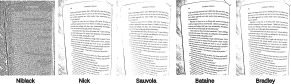
\includegraphics[width=\textwidth]{graphics/Window7x7}
    \caption{Qualitative comparison of the evaluated thresholding approaches using a $7\times 7$ window size.}
    \label{fig:window_sizes}
\end{figure*}

\subsection{Modern Approaches}\label{subsec:modern}

In addition to the classical local thresholding methods derived from Niblack's formulation~\cite{Niblack1985}, we also investigate two more recent adaptive binarization approaches that emphasize computational efficiency and robustness under challenging illumination conditions.

% Integral Image: Fast Mean-Based Approach
\paragraph{Integral-Image-Based Thresholding.}
Bradley and Roth~\cite{Bradley2007} propose a fast adaptive thresholding technique based on integral images.
The central idea is to compute local mean pixel values (intensities) efficiently by using a cumulative sum representation.

% Integral Processing
Given an image $f(x,y)$, the integral image $S(x,y)$ is defined as 

\begin{equation}
  S(x,y) = \sum_{i=0}^{x} \sum_{j=0}^{y} f(i,j).
\end{equation}

Using this representation, the sum of intensities within any rectangular window can be obtained in constant time, independent of the window size.
This significantly reduces the computational cost of sliding-window thresholding.

The method compares each pixel value against the average intensity of its surrounding $s \times s$ neighborhood.
A pixel is classified as foreground if its intensity is at least $t$ percent lower than the local mean.
Otherwise, it is assigned to the background.
The overall procedure consists of the following steps:

\begin{enumerate}
  \item Compute the integral image representation of the input.
  \item Apply the adaptive mean-based threshold to produce the binarized output.
\end{enumerate}

% Bataineh: Naive Local Statistics Approach
\paragraph{Adaptive Statistics Thresholding.}
Bataineh et al.~\cite{Bataineh2011} introduce an adaptive thresholding approach that incorporates both local and global image statistics. 
In contrast to purely mean-based methods, their formulation adjusts the threshold using an adaptive standard deviation term derived from local window variations.

The threshold is defined as

\begin{equation}
  T = m_W - \frac{m^2_W - \sigma_W}{(m_g + \sigma_W) \times (\sigma_{\text{Adaptive}} + \sigma_W)} ,
\end{equation}

where $m_W$ and $\sigma_W$ denote the mean and standard deviation within the current window, and $m_g$ is the global mean intensity of the entire image.

The adaptive standard deviation is computed as a normalized measure of local contrast:

\begin{equation}
  \sigma_{\text{Adaptive}} = \frac{\sigma_W - \sigma_{\min}}{\sigma_{\max} - \sigma_{\min}},
\end{equation}

where $\sigma_{\min}$ and $\sigma_{\max}$ represent the minimum and maximum window standard deviations observed across the image.
This normalization allows the method to adjust the threshold dynamically depending on the degree of local variation.

\subsection{Performance Optimization}\label{subsec:optimizations}

In addition to evaluation denoising quality, we place strong emphasis on computational efficiency.
Many adaptive thresholding techniques require the computation of local statistics over sliding windows, which can become a major performance bottleneck for high-resolution images.
To systematically improve runtime performance, we applied profiling guided optimizations using the \textit{Instruments} profiler on macOS.
To illustrate this process, we focus on the implementation of the adaptive thresholding method proposed by Bataineh et al.~\cite{Bataineh2011}.

% \paragraph{Baseline Window Computation.}
Our initial baseline implementation followed the direct formulation of the algorithms, computing the local mean and standard deviation independently for each pixel by explicitly iterating over all pixels within the corresponding window.
Due to overlapping neighborhoods, this approach performs a large number of redundant computations and scales poorly with increasing window size.

% \paragraph{Reduced Window Computations.}
As a first optimization, we reformulated the variance computation to obtain both the mean and standard deviation in a single window pass by accumulating the sum of pixel and squared pixel values.
This reduces constant overhead and preserves the original thresholding formulation. 

% \paragraph{Integral Image Acceleration.}
A more substantial improvement was achieved by adopting integral image representations. 
This optimization reduces the overall computational complexity of window-based thresholding from quadratic to linear in the number of pixels.

% \paragraph{Parallel Execution.}
Finally, we explored parallel implementations using OpenMP.
Since threshold computations are independent for each pixel, the algorithms exhibit a high degree of data parallelism.
Parallel execution may therefore provide additional runtime improvements on multicore architectures.

Together, these optimizations significantly reduce execution time while maintaining the denoising effectiveness of the underlying adaptive thresholding approach.


%--------------------------------------------%
% EXPERIMENTS AND RESULTS -------------------%
%--------------------------------------------%
\section{Experiments and Results}\label{sec:experiments_results}

We conducted a series of experiments to evaluate both the effectiveness and computational efficiency of the implemented denoising and binarization approaches.
Since all methods rely on local statistics computed over sliding windows, we analyze the influence of different window sizes on the resulting binarization quality.
In addition, we compare the runtime performance of the considered approaches in order to assess the impact of the proposed implementation and optimization strategies.

\subsection{Experimental Setup}\label{subsec:exp_setup}

Experiments were performed on two representative test images of different resolutions.
A medium-sized image of resolution $736 \times 981$ pixels was used primarily for qualitative comparison, as it allows clear visual assessment of binarization quality.
In addition, a high-resolution image of size $6700 \times 4467$ pixels was used for performance benchmarking in order to analyze the runtime behavior under computationally demanding conditions.

All images were converted to grayscale using the preprocessing procedure described in Section~\ref{sec:ATA}.
We evaluate the classical local thresholding methods as well as the more recent adaptive approaches.
For all window-based techniques, we test multiple neighborhood sizes ($7\times 7$, $15\times 15$ and $21\times 21$) to study the effect of window size on robustness and output quality.
Runtime measurements are reported for the high-resolution image to highlight the impact of integral-image acceleration and parallelization.


% Figure 2: One approach for the different window sizes
\begin{figure}[t]
    \centering
    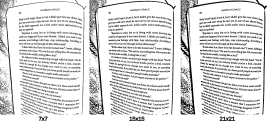
\includegraphics[width=\linewidth]{graphics/BatainehWindowSizes}
    \caption{Binarization results of Bataineh's method for different window sizes ($7\times 7$, $15\times 15$, and $21\times 21$).}
    \label{fig:bataineh_window_sizes}
\end{figure}

\subsection{Qualitative Comparison}\label{subsec:qualitative_compare}

Figure~\ref{fig:window_sizes} presents the binarization results obtained with the different adaptive thresholding methods for a window size of $7\times 7$.
Overall, most approaches are able to separate foreground text from the noisy background, although notable differences in robustness and visual clarity can be observed.

% 7x7
For the smallest window size, Niblack's method produces the most distinct output. 
While the algorithm captures the textual structures reasonably well, it fails to suppress background noise effectively, leading to reduced contrast between the text in the image (foreground) and background.
Sauvola's method improves upon this behavior but still exhibits occasional inaccuracies in low-contrast regions.
In contrast, the Nick approach yields cleaner results despite being closely related to the Niblack and Sauvola formulations, indicating improved robustness of its modified threshold computation.
Among all methods Bradley's integral image based approach achieves the clearest separation ot text from background, producing the most visually consistent binarization. 

% 15x15
Increasing the window size to $15\times 15$ does not fundamentally change the relative performance of the methods, but it affects the amount of remaining background artifacts.
In particular, the modern approaches by Bradley and Bataineh tend to produce thicker character strokes and more pronounced contours.
Niblack's method benefits from the larger neighborhood, showing improved foreground-background separation compared to the $7\times 7$ case, although background noise remains more prominent than for the other approaches.

% 21x21 
For the largest evaluated window size of $21\times 21$, these effects become even more pronounced. 
While Niblack continues to improve in separating text from background, the output of Bataineh's method increasingly includes bold foreground structures as well as additional background contours.
This behavior is illustrated in Figure~\ref{fig:bataineh_window_sizes}, where larger windows lead to stronger stroke widths. 

Overall, Bradley's approach appears least sensitive to different window sizes, providing consistently high-quality binarization across all evaluated configurations.
Bataineh's method achieves strong contrast but requires careful parameter selection, whereas the classical methods show moderate improvements with increasing window size but remain less robust under heavy noise.

\subsection{Runtime Performance}\label{subsec:runtime_perf}

For the evaluation of the computational efficiency of the implemented approaches, we examine the runtime impact of the optimizations described in Section~\ref{subsec:optimizations}.

\paragraph{Optimization Impact.}
Table~\ref{tab:table_bataineh} summarizes the progressive runtime improvements obtained for the method of Bataineh et al.~\cite{Bataineh2011}.
Starting from a naive baseline implementation with explicit sliding-window computations, successive optimizations significantly reduced the execution time.

% Table 1: Compares different optimizations for Bataineh's approach
\begin{table}[t]
    \begin{tabular}{lcccc}
                  & Base & Single-Pass & Integral Image & OpenMP \\
        \hline
        Time (ms) & 1330 & 748         & 188            & 195
    \end{tabular}
    \caption{Runtime comparison of optimization stages for Bataineh's method on the medium-resolution image.}
    \label{tab:table_bataineh}
\end{table}

The results demonstrate that algorithmic improvements, particularly the use of integral images, provide the largest performance gain.
Overall, the optimized implementation achieves an approximate $7\times$ speedup compared to the baseline.
Interestingly, the OpenMP parallelized version does not yield further improvement, suggesting that the computation becomes limited by memory access overhead and parallelization costs rather than arithmetic operations.

\paragraph{High-Resolution Image Runtime.}
To better distinguish the performance characteristics of the different approaches, we also benchmarked all optimized methods on a high-resolution image of size $6700 \times 4467$ pixels.
The resulting runtimes are reported in Table~\ref{tab:table_compare}.

% Table 2: Comparing the different approaches on a 4K picture
\begin{table}[t]
    \begin{tabular}{lc}
        Approach & Time (s) \\
        \hline
        Niblack  & 6.30 \\
        Sauvola  & 6.44 \\
        Nick     & 6.34 \\
        Bataineh & 6.39 \\
        Bradley  & 4.55 
    \end{tabular}
    \caption{Running times of the optimized approaches on the high-resolution image.}
    \label{tab:table_compare}
\end{table}

All classical window-based methods exhibit similar runtime behavior, as they require both mean and standard deviation statistics for each pixel.
Bradley's approach achieves the lowest runtime, which can be attributed to its reliance on mean-based thresholding only, combined with the efficiency of integral image evaluation.


%--------------------------------------------%
% CONCLUSION --------------------------------%
%--------------------------------------------%
\section{Conclusions}\label{sec:conclusion}

We investigated several established and modern adaptive thresholding techniques for the denoising and binarization of noisy color images, with a particular focus on efficient processing of PPM image data.
All methods were implemented according to their original formulations and evaluated with respect to both binarization quality and computational performance.

Our qualitative experiments show that classical approaches such as Niblack and Sauvola provide reasonable results but are less robust to background noise compared to more recent methods.
The Nick method improves upon these baselines, while the approaches of Bataineh and Bradley achieve the highest visual quality.
Bradley's method in particular produces the most consistent foreground-background separation across different window sizes.

In terms of efficiency, profiling-guided optimizations demonstrate that the computation of local window statistics is the dominant performance factor.
Integral image based implementations substantially reduce redundant calculations and provide significant runtime improvements, especially for high-resolution images.
Overall, our results highlight the importance of combining adaptive thresholding formulations with efficient implementation strategies.


%--------------------------------------------%
% BIBLIOGRAPHY ------------------------------%
%--------------------------------------------%

%% The next two lines define the bibliography style to be used, and
%% the bibliography file.
\bibliographystyle{ACM-Reference-Format}
\bibliography{literature}


\end{document}
\endinput
%%
%% End of file `sample-sigconf.tex'.
